\documentclass[conference]{IEEEtran}
\IEEEoverridecommandlockouts
% The preceding line is only needed to identify funding in the first footnote. If that is unneeded, please comment it out.
\usepackage{cite}
\usepackage{amsmath,amssymb,amsfonts}
\usepackage{algorithmic}
\usepackage{graphicx}
\usepackage{textcomp}
\usepackage{xcolor}
\usepackage{float}
\def\BibTeX{{\rm B\kern-.05em{\sc i\kern-.025em b}\kern-.08em
    T\kern-.1667em\lower.7ex\hbox{E}\kern-.125emX}}
\begin{document}

\title{MRI Documentation\\
{\footnotesize MRI and its Components: A concept}
}

\author{\IEEEauthorblockN{Carl-Georg Meyer}
\IEEEauthorblockA{\textit{Electronic Engineering} \\
\textit{HSHL Hamm-Lippstadt}\\
Lippstadt, Germany \\
carl-georg.meyer@stud.hshl.de}

}

\maketitle

\begin{abstract}
MRI-Systems play a crucial role in the field of radiology in the medical domain. A concept was to be designed with concrete components selected. This was successfully done with an architecture and hardware requirements able to be defined. A user interface was also created to get a greater understanding. To finalize a conclusion and outlook was reached.
\end{abstract}

\begin{IEEEkeywords}
HSHL, MRI, Interactive, Engineering, Interactive Systems Engineering, Electronic Engineering
\end{IEEEkeywords}
\tableofcontents
\section{Introduction}
    
    
    This documentation is done as part of the Interactive Systems Engineering module at the Hochschule Hamm-Lippstadt. Our task was it to conceptualise a medical system, which is able to monitor vital signs, detect anomalies, alarms and has a user interface.
    I selected an Magnetic resonance imaging (MRI) system to develop a concept for. It is a technology used in the radiology part of the medical domain and is used to scan the human body for anomalies using electro-magnetic fields.
    The intention behind that lies within a family member being partially disabled and having had multiple visits to the hospital for MRI scans, specifically the brain. Therefore I saw this as an opportunity to get more knowledge of the technology and combine that with the knowledge gained from the Electronic Engineering course of study. Additionally the problem arose to either simply or improve upon current MRI-System, which played a factor in me choosing this system.
    In this paper is structured in two parts, with the first initially talking about the concept itself. Following that will be the design of the concept which talks a bit more detailed about the requirements, models and components of the system, concluding with the user interface. The second half of the paper will deal with a reflection of the system, seeing what it covers so far and if it solved the initial problem. The paper then concludes with a summary and outlook.
    


\section{Concept}

    For the concept of the MRI-System it was important to simplify the system into its most basic parts and then use that as a base to create an architecture.

    The architecture of the system is working in the following way (see Fig.1. for reference):

    The medical staff, in this case the doctor, makes inputs through the input device which are then read out by the CPU. Following this the CPU will then control the bed with the patient on it and send/receive data to or from the magnet and gradient coil. Data received is then stored on the storage device and server, whilst being send to the output device. From that the medical staff can then read out information and make new inputs.

    \begin{figure}[htbp]
    \centerline{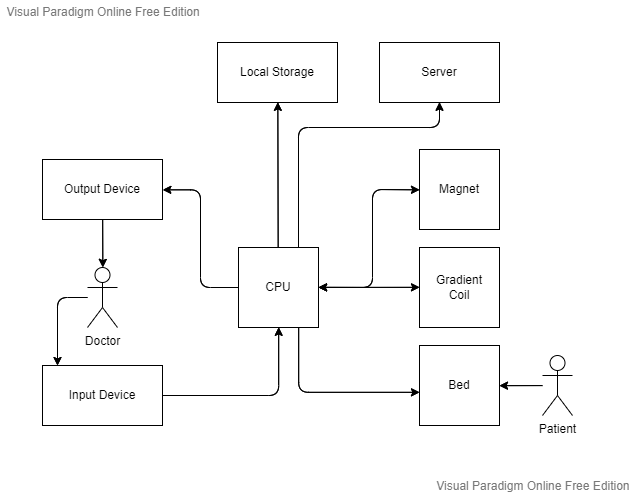
\includegraphics[scale = 0.4]{Pictures/blockdiag.png}}
    \caption{Block Diagram}
    \label{block}
    \end{figure}

    With the architecture of the system described it is also important to briefly show the work flow of the system and how a procedure would look like. The procedure works in the following steps:
    
    \begin{enumerate}
        \item System idles
        \item Patient lays down on the bed
        \item Doctor moves the bed via the computer
        \item Doctor makes inputs into the system
        \item Computer then converts those inputs to the machine
        \item Scan begins
        \item Data is being processed
        \item Processed data is shown to doctor and communicates with the patient
        \item Scan stops
        \item Bed is being moved to a new position
        \item Loop scanning until done
        \item Doctor moves bed back to initial position
        \item System is back to idling
        \item Patient is able to get up from the bed and is able to leave
    \end{enumerate}
    

\section{Design of concept}

    \subsection{Requirements}
    
    This section deals with the hardware requirements for the system. Each requirement is giving a short title description and to what component it is related to.
    
    \begin{enumerate}
        \item   HR1: Create magnetic field\newline
                Description:	System must create a magnetic field in order to scan the subject.\newline
                Relation:	Magnet, Gradient Coils
        \item   HR2: Process images\newline
                Description:    System must be able to convert received data into viewable data.\newline
                Relation:	Image Processing
    
        \item   HR3: Display Images\newline
                Description:	System must visualize viewable data.\newline
                Relation:	Image Processing
    
        \item   HR4: Power\newline
                Description:	System must create and maintain enough power for the system to run as designed.\newline
                    Relation:	MRI RF Power Amplifier Module
    
        \item   HR5: Movable bed\newline
                Description:	System must be able to move bed for the patient.\newline
                Relation:	MRI subsystem Module
    
        \item   HR6: Receive Data\newline
                Description:	System must be able to receive data in order to convert them.\newline
                Relation:	MRI Receive Module
    
        \item   HR7: Input\newline
                Description:	System must have an input method like a keyboard and mouse.\newline
                Relation: 	Input Device
    
        \item   HR8: Storage\newline
                Description:	System must storage data on a storage device.\newline
                Relation:	Storage Device, Server
    \end{enumerate}
    
    
    \subsection{Models}
    
    Now that the hardware requirements are defined it is also important to look at the corresponding models to get a greater understanding of the entire system. This is done by firstly talking about the state machine diagram, followed by the use case and lastly activity diagram.
    
    \subsubsection{State Machine Diagram}
    
    This diagram describes the different states the system can be in. Initially it is in the idle state and awaits inputs from the person operating the system. It then remain idle unless a scan is being performed, in which case it switches to the active state. This one can either be canceled or completed. Should an emergency occur, the system then moves into the fail-safe state and eventually shuts down. Both outcomes lead to the system resuming the idle state. The system can also be serviced in which case it moves to the out of service state and back to idle once it is fixed.
    
    \begin{figure}[htbp]
    \centerline{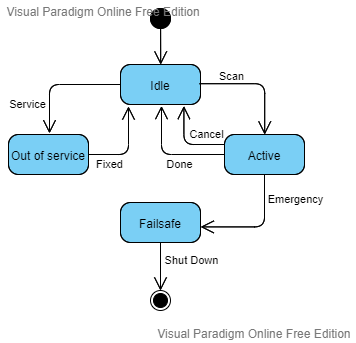
\includegraphics[scale = 0.62]{Pictures/statemachine.png}}
    \caption{State Machine Diagram}
    \label{statemachine}
    \end{figure}
    
    \subsubsection{Use Case Diagram}
    
    For the Use-Case-Diagram we have 3 actors and 10 possible use-cases. The actors are the doctor, patient and technician.
    The patient only has to lay down as the more detailed procedure for them is described in the Activity-Diagram in 5.3.
    The technicians use-cases describe the general maintenance and repair of the system. This is crucial to keep the system running flawlessly and ensure that in case of a failure that it is brought back to a state of operability.
    The Doctor plays the most important part as they are the ones operating the system. Therefore they are able to control the system as a whole, which is represented in their ability to scan the patient or move the bed. Additionally they can view the scanned images in real time and control the images that are being displayed. Lastly they have control over the radio frequencies (RF) and can make other minor inputs. Another minor adjustment they can make is the way images may be processed.
    
    \begin{figure}[htbp]
    \centerline{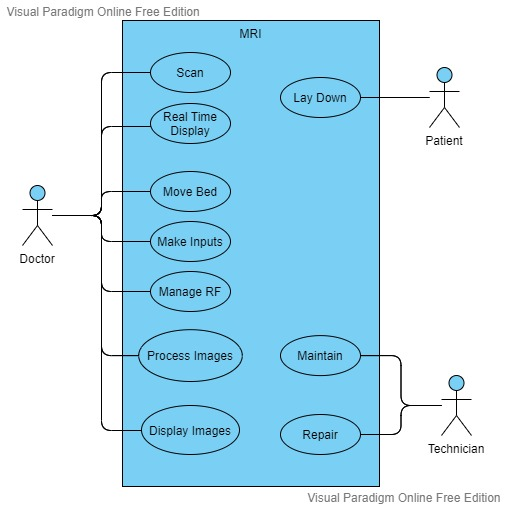
\includegraphics[scale = 0.5]{Pictures/mri_usecase.jpg}}
    \caption{Use Case Diagram}
    \label{usecase}
    \end{figure}
    
    \subsubsection{Patient Activity Diagram}
    
    Initially the patient lays down on the bed of the MRI and gets comfortable to begin the procedure. They can adjust themselves and have to keep their arms on their body. After that the bed begins to move and is brought into position for the scanning procedure to begin. A scan is then started and completed and a decision has to be made to either continue scanning or if the scanning is complete. Should more scans be necessary the bed moves to a new position and the scanning continues. If it is then decided that the scanning has finished the bed is moved back to its initial position and the patient is able to stand up and leave.
    
    \begin{figure}[htbp]
    \centerline{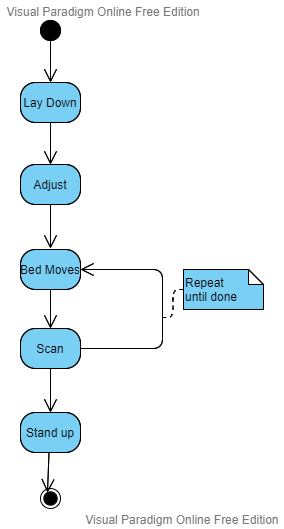
\includegraphics[scale = 0.5]{Pictures/actyp.png}}
    \caption{Patient Activity Diagram}
    \label{activity}
    \end{figure}   
    
    
    
    \subsection{Components}
    
    In this part of the design section the components of the system will be introduced, explained. In some cases where it is reasonable, some suggestions for the hardware are being made. Overall it is difficult to get precise component listed due to manufactures being very confidential with the actual components used. So the suggestions are meant as such and not definitive solutions.
    
    \subsubsection{Magnet}

        The magnet is the most expensive part of the entire system. The current standard for magnets is to use ones which are superconductive. Reason being is that there a lot of applications for such magnets which makes them very desirable. Where before with water cooled resistive magnets the magnetic field was limited to around 0.3T (T = Tesla, the unit to measure magnetic fields), superconductive magnets can achieve up to 4.0T. This in the end allows a full body scan \cite{fmrib}.

    \subsubsection{Gradient Coil}
    
        The gradient coil needs to accomplish two things. Firstly it needs to “produce a linear variation in field along one direction” \cite{fmrib} and secondly to have “high efficiency, low inductance and low resistance” \cite{fmrib}. This has to be done to minimize heat deposition and the requirements regarding currents.
        When talking about gradient coil in terms of an MRI, a specific type of coil called “Maxwell coil” is being used. Their characteristics are that they consist of a pair of coils which are being separated by 1.73 times their radius. Current then flows through in the opposite sense in the two coils, which then generates the linear gradient \cite{fmrib}.
    
    
    \subsubsection{Control and Processing}
    
        The control of the whole system is handled by a central computer, as well as the processing. It is able to specify the shape of the RF-waveform and the timings that are meant to be used during the scanning process. A possible part of the computer can be the
        
        \begin{itemize}
            \item AM2732 Dual-core Arm® Cortex-R5F based MCU with C66x DSP, ethernet and security up to 400 MHz \cite{AM2732}\cite{sheet}
        \end{itemize}    

        by Texas instruments. It would be a viable choice due to its two integrated CPUs and rating for security applications \cite{fmrib}.
          
    
    
    \subsubsection{Image Processing}
    
        Image Processing is one of the most elementary parts of the whole MRI-System, since without it a medical analysis is impossible. To do this effectively a number of components is required to make this possible. These are in no particular order:
        
        \begin{itemize}
            \item 12-Bit, 1.5Gsps High-Dynamic Performance DAC \cite{MAX19681}
            \item High-Dynamic-Range, 16-Bit, 100Msps ADC with -82dBFS Noise Floor \cite{MAX19588}
            \item Ultra-Low-Power, 8-Channel, 12-Bit, 64Msps ADC \cite{MAX19528}
            \item Ultra-Low-Power, Octal, 12-Bit, 50Msps, 1.8V ADC with Serial LVDS Outputs \cite{MAX19527}
            \item Ultra-Low-Power, 8-Channel, 12-Bit, 40Msps ADC \cite{MAX19526}
        \end{itemize}    

    \subsubsection{Integrated Circuits}      

        Integrated circuits also play a role in the design of an MRI-System. They are able to accomplish specific tasks which lead to better results in the scanning process. The three modules listed below combined accomplish optimized coil and gradient performance, which leads to enhanced diagnostic capabilities.
        In addition to that, MRI-System often require “precise control of the magnetic and radio frequency field in the system”, “reduced scan time and improved form factor to enhance patient comfort” as well as “optimized power consumption and cloud connectivity” \cite{RFRM}\cite{RFPAM}\cite{RFSSM}.
        It also makes sense to choose those modules do to their shared technologies. They are each powered by their own power supply and possess input protection. Both things helping with the security of the entire system. Tasks like line protection, clocking or gradient control is covered by multiple modules, enabling redundancy. Below is a simplified list of the components of each module, with previously mentioned components not listed.
        
        \begin{itemize}
            \item MRI Receive Module \cite{RFRM}\newline
                    Receive signal chain\newline
                    Digital processing\newline
                    Receive line input
            \item MRI RF Power Amplifier Module \cite{RFPAM}\newline
                    Transmit signal chain\newline
                    Digital processing
            \item MRI subsystem Module \cite{RFSSM}\newline
                    Diagnostics\newline
                    Gas sensor front-end\newline
                    Digital processing\newline
                    Transmit and receive signal chain\newline
                    Motor drive\newline
                    Drive MCU\newline
                    Current Sensing\newline
                    Analog or digital position sensing for motor\newline
                    Input user interface\newline
                    Wired interface\newline
                    Memory\newline
                    Clocking\newline
                    Output user interface
        \end{itemize}    

        
    \subsubsection{Storage Device}

    Storage plays a minor factor in the entire system, but is nonetheless important. This is because it serves as a place for the doctor to access the processed pictures from, but also a medium to save them on. In addition to that it plays a factor in building a permanent back-up that can be stored on the hospitals server. Lastly it is common practice to give the patient a CD with all the pictures included so it makes sense that a storage device of at least 20GB. It also makes sense to use an NVMe SSD or SSD over an HDD due to the speed difference. A possible solution could be:
        
        \begin{itemize}
            \item 850 EVO SATA III 2.5zoll SSD \cite{SSD}
        \end{itemize}   
        
    \subsubsection{Server}

    To back up and save data in the long term it makes sense that system is connected to a server. This way it can be ensured that data of multiple patients can be saved for multiple years and it is not required for the patient to bring their physical copy to each appointment after the scan.
    It would therefore make sense to use a local server directly at the hospital. The main benefits being that it can be connected from the MRI-System through an intranet connection, which adds another layer of security, but also to the internet so medical personal can access it when they are not directly in the hospital themselves.
    Alternatively the server space could be bought from service providers like AWS S3, but that might not be cost efficient in the long term. Pricing for an AWS S3 solution would look something like this:
        
        \begin{itemize}
            \item Storage cost: charged per GB / month. $\sim$ \$0.03 / GB / month, charged hourly
            \item API cost for operation of files: $\sim$ \$0.005 / 10000 read requests, write requests are 10 times more expensive
            \item Data transfer outside of AWS region: $\sim$ \$0.02 / GB to different AWS region, $\sim$ \$0.06 / GB to the internet \cite{AWS}
        \end{itemize}    

    Overall a server adds another point of redundancy since the desired data is now available at two points.
    
    \subsection{User Interface}

    The user interface is solely directed towards the medical staff and is therefore designed in a way that requires an understanding of the machine and human body.
    In the top row of the UI are multiple options to choose from, which are Patient, Application, Tools, View, System, Options and Help. The first four options are specifically designed for the medical staff. The patient options gives them more information on the patient, application lets the staff choose which part of the body is to be scanned and can therefore fine tune the scanning. Tools give the staff more options during the procedure, like scanning range. View lets the staff look at the live scan or switch to previous scans.
    System, Options and Help are designed for the staff and technician in mind. System gives the technician a more technical look at the system to either fix or maintain the system, where as Options and Help are there to change things like the language and give user manual in case of uncertainty.
    Below that is the main image of the current scan. It is large so multiple angles of the human body can be displayed in a detailed manner. In the bottom right corner is a visualization of the parts that are being scanned by the system currently. Blue boxes mark the scanned and black boxes mark the non-scanned areas. There are also changeable parameters in that section.
    To the lest is the scanning range. This works in conjunction with the area in the bottom right to make fine tuned adjustments during the scanning process.
    Last but not least are multiple buttons in the bottom left. These are play, pause, skip, stop and a microphone. Their main function is it to watch the scan in a time-lapse fashion and to be able to communicate to with the patient. An example can be found in the appendix.

\section{Discussion}

    Currently this concept covers all the basic functions of an MRI-System and would be able to be used in a hospital or radiological environment.
    Overall the initial problem has been solved, as a complete MRI-System was able to be conceptualized with all the key elements in it.
    Things like the UI and system architecture were things that improved as lectures took place. Especially the UI went through multiple iterations to cater towards professionals whilst also being easy to understand, simple and compact. Talking about the architecture, this also when through multiple versions to talk things like redundancy and simplicity into account and still being scientifically accurate.
    

\section{Conclusion}

    \subsection{Summary}
    
    To summarize, it was the task to create a medical device that is able to monitor vital signs and I chose to realize that with an MRI solution. This has been successful since a full concept for the system was able to be designed with concrete models and hardware. Requirements for the system were also able to be established successfully with direct suggestions for hardware given. Since the whole MRI-system is a big sensor it was able to fulfill that criteria as well.    
    
    \subsection{Outlook}
    
    In the future the concept can be further expanded upon as more knowledge is able to be gained about it. Things like more concrete hardware solutions and safety critical hard- and software might be able to be found and implemented. Furthermore MRI-System technologies will continue to be developed so the concept will evolve alongside those system. This will lead to more safety for the patient, faster procedures and less energy consumption for the whole system, making it more environmentally friendly in the context of a hospitals power consumption.

\bibliographystyle{plain}
\bibliography{mybibfile}
\clearpage
\onecolumn
\appendix

    \begin{figure}[htbp]
    \centerline{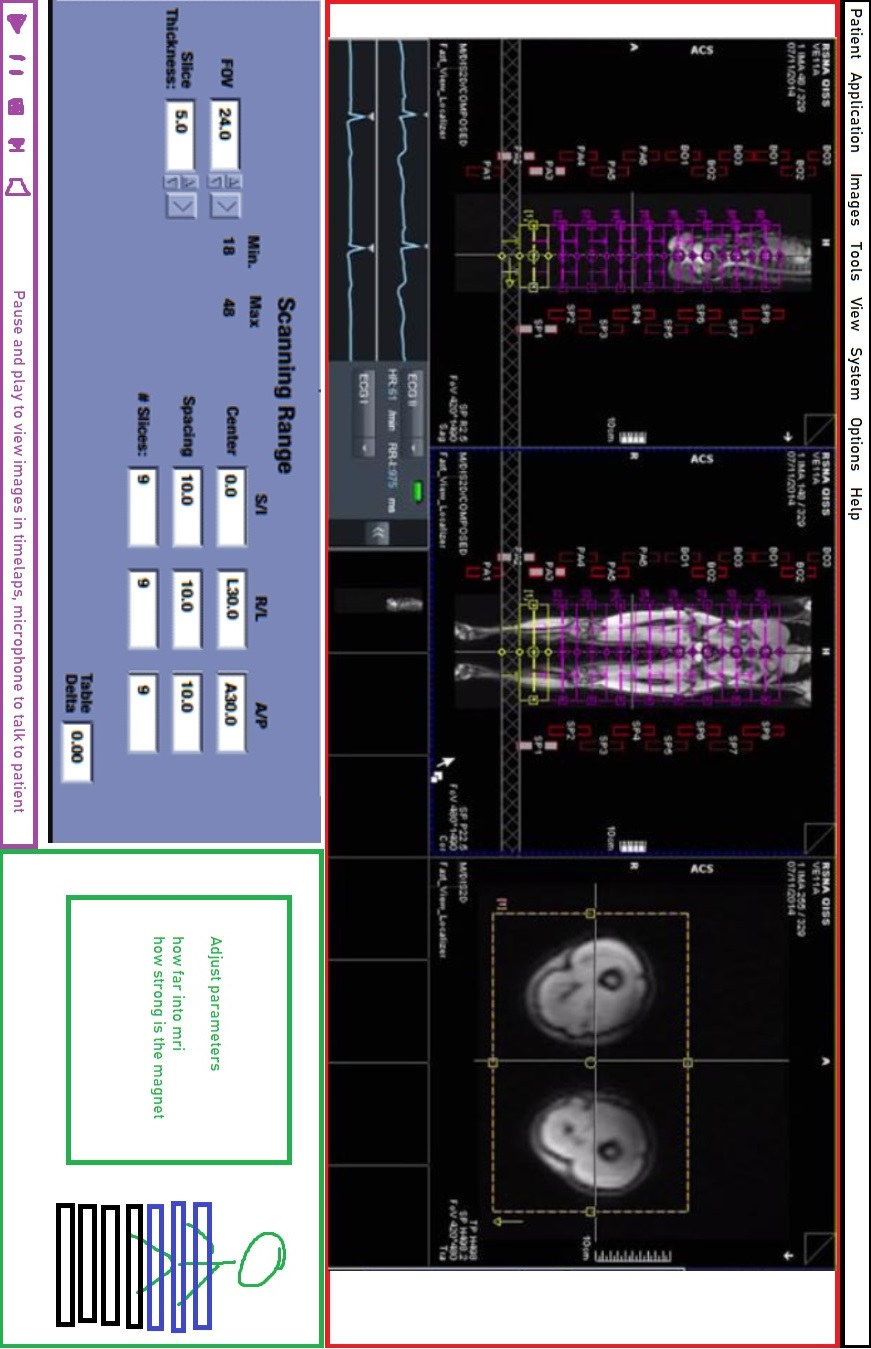
\includegraphics[scale = 0.56]{Pictures/badui.jpg}}
    \caption{User Interface}
    \label{UI}
    \end{figure}   
    
\end{document}
